\documentclass[aps,reprint]{revtex4-2}
%\documentclass[aps,pre,twocolumn,showpacs,floatfix]{revtex4-2}

\usepackage{graphicx}
\usepackage{booktabs}
\usepackage{amsmath}

\begin{document}

\title{Dynamic Strangle as a Lossless Hedge}
\author{Steve Drasco}
\affiliation{Independent Researcher}
\email{steve.drasco@gmail.com}
\date{\today}

\begin{abstract}
Purchasing a call and a put contract on the same underlying generally produces a “well-shaped” profit-and-loss curve with a loss at the center and profit emerging on either side beyond two breakeven points. For fixed premiums, one could in principle reposition the strikes to invert these breakeven points, raising the well and eliminating loss. This brief note examines how realistic, variable premiums affect such an approach, showing that a truly lossless configuration generally requires the two contracts to be acquired at different times under very different market conditions. For sufficiently large differences in the underlying prices at the times of purchase, this mechanism can provide a lossless hedge for a position that has developed into deep in-the-money status.
\end{abstract}

\maketitle

\section{Overview}

This short note explores the risk associated with a novel position resembling the familiar strangle.  The aim is to find conditions for an arbitrage or lossless position.  To fix notation we begin with a reminder of the profit/loss curves for a long put, a long call, and their combination in a strangle. 

A \textbf{long put} with strike price $K_P$ and premium $P$ has profit/loss $\varphi_P$ as a function of underlying asset price $S$
\begin{equation}
\varphi_P(S) = \max(K_P - S,\,0) - P~,
\end{equation}
sketched in Fig.~\ref{fig:put}.
\begin{figure}[hb]
    \centering
    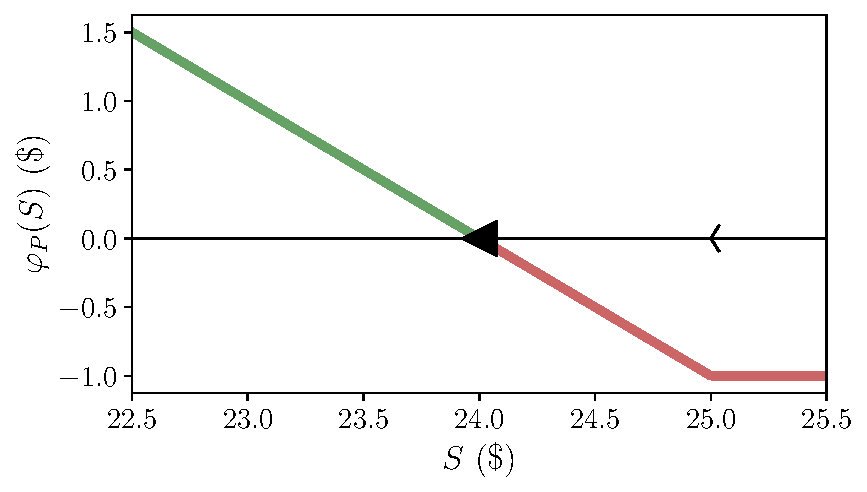
\includegraphics[width=0.45\textwidth]{figs/put.pdf}
    \caption{Profit and loss curve for a long put with representative values of $K_P = \$25$ and $P = \$1$.  The breakeven point $S_- = K_P - P$, is shown as a left-pointing triangle.}
    \label{fig:put}
\end{figure}

If $S > K_P$, at the time of exercising, the option finishes worthless,  and the net loss is the premium $P$. If instead $S<K_P$, the profit increases linearly as $S$ decreases, bounded by $\varphi_P(0) = S_-$, where 
$S_-$ is also the breakeven point for the put
\begin{equation}
S_- = K_P - P~.
\end{equation}


A \textbf{long call} with strike price $K_C$ and premium $C$ has profit/loss 
\begin{equation}
\varphi_C(S) = \max(S - K_C,\,0) - C~,
\end{equation}
sketched in Fig.~\ref{fig:call}.
\begin{figure}[hb]
    \centering
    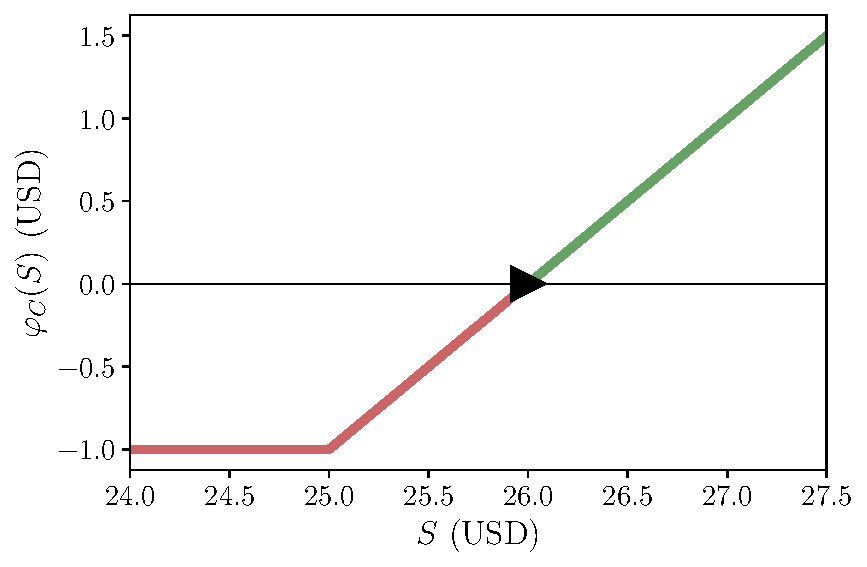
\includegraphics[width=0.45\textwidth]{figs/call.pdf}
    \caption{Profit and loss curve for a long call with representative values of $K_C = \$25$ and $C = \$1$.  The breakeven point $S_+ = K_C + C$, is shown as a right-pointing triangle.
    }
    \label{fig:call}
\end{figure}

If $S < K_C$ at the time of exercising, the call is worthless and the net loss is the premium $C$. If instead $S>K_C$, the net profit increases
linearly with $S$, without bound. The breakeven point for the call occurs at underlying price
\begin{equation}
S_+ = K_C + C~.
\end{equation}

A \textbf{strangle} combines a long put and a long call giving a total profit/loss
$\varphi(S)= \varphi_P(S) + \varphi_C(S)$,
\begin{equation}
\varphi(S) = \max(K_P - S,\,0) + \max(S - K_C,\,0) - \Pi~,
\end{equation}
with total premium $\Pi = P + C$.  
A generic strangle with $K_P < K_C$, is sketched in Fig.~\ref{fig:strangle}.
\begin{figure}[hb]
    \centering
    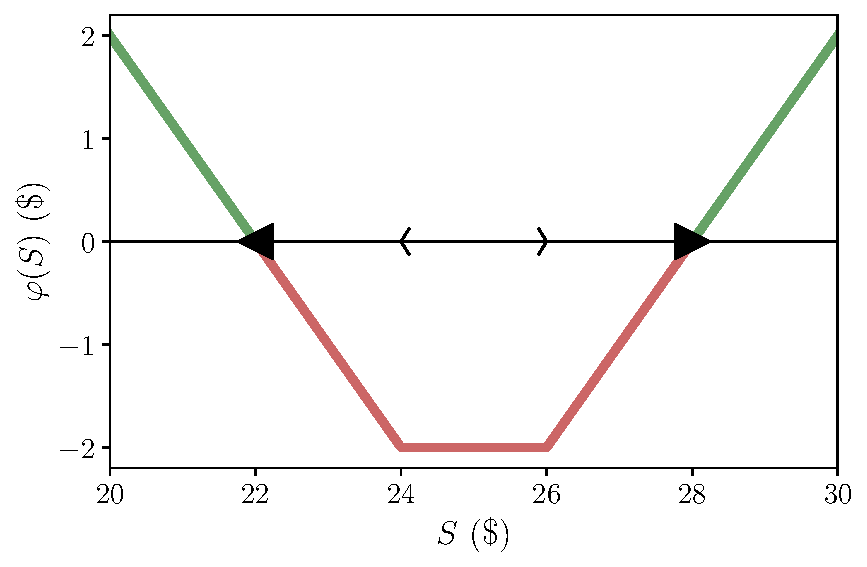
\includegraphics[width=0.45\textwidth]{figs/strangle.pdf}
    \caption{Profit and loss curve for a generic strangle with representative values
    $K_P = \$24$, $K_C = \$26$, and $C = P = \$1$.
    The breakeven points $S_\pm$ are again shown as triangles.}
    \label{fig:strangle}
\end{figure}
This produces a profit when $S$ moves significantly outside the strike region $(K_P, K_C)$, but has a loss in the middle. 
The two breakeven points for this strangle are
\begin{equation}
S_{-} = K_P - \Pi~, 
\quad 
S_{+} = K_C + \Pi~.
\end{equation}
If $K_P < K_C$, then $S_{-} < S_{+}$.  When $K_P > K_C$ however, it is possible to have inverted breakeven points $S_{-} > S_{+}$.

This note explores the feasibility of a strangle position whose profit/loss curve is raised in such a way that the loss well is entirely eliminated,  $\varphi(S) \geq 0$ for all $S$. 

\section{Fixed premium model}

We begin by assuming, unrealistically, that the strikes can be adjusted without changing the total premium 
\begin{equation}
\Pi = P + C~.
\end{equation}
The sequence shown in Fig.~\ref{fig:sequence} demonstrates the effect of shifting the strikes $K_C$ and/or $K_P$,  in such a way that 
its breakeven points are inverted $S_- \geq S_+$, and  $\varphi(S) \geq 0$, for all $S$.
\begin{figure*}[hb]
    \centering
    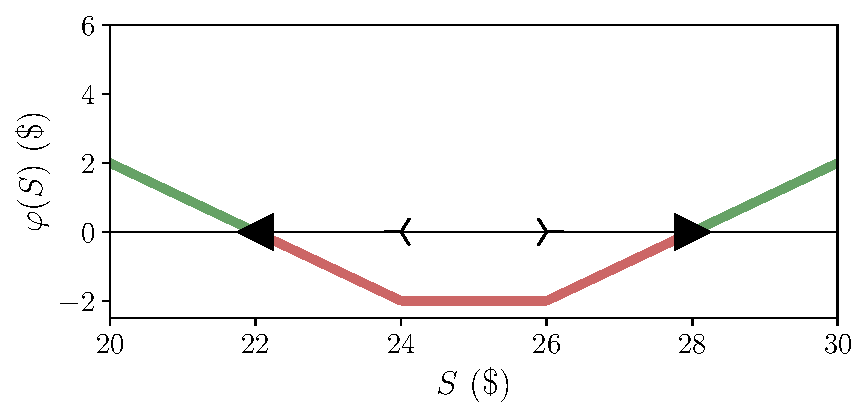
\includegraphics[width=0.3\textwidth]{figs/sequence1.pdf}
    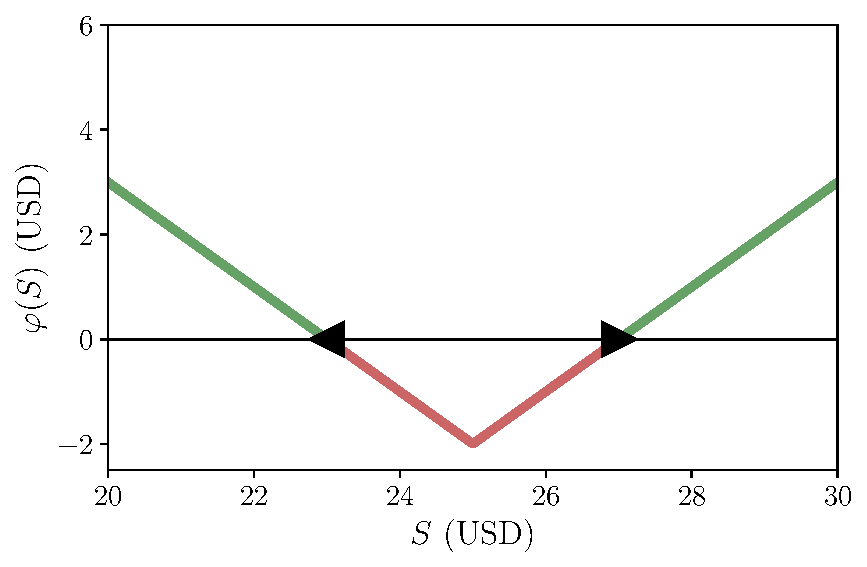
\includegraphics[width=0.3\textwidth]{figs/sequence2.pdf}
    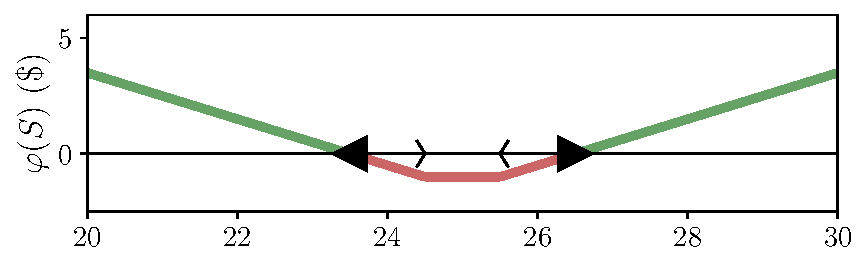
\includegraphics[width=0.3\textwidth]{figs/sequence3.pdf}
    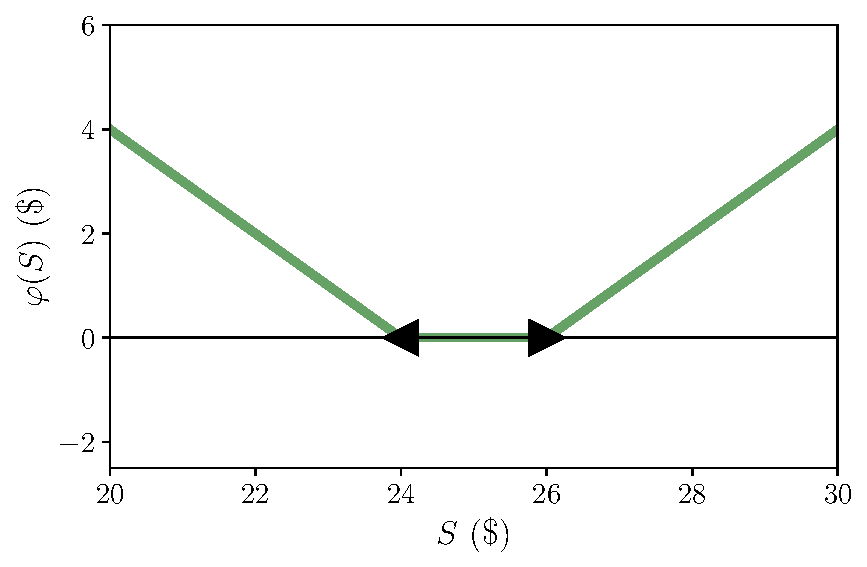
\includegraphics[width=0.3\textwidth]{figs/sequence4.pdf}
    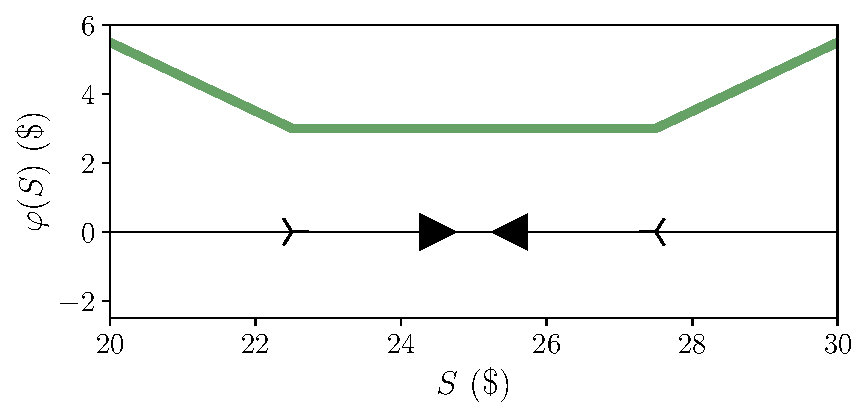
\includegraphics[width=0.3\textwidth]{figs/sequence5.pdf}
\caption{
    A sequence of profit and loss curves as strikes $K_C$ and/or $K_P$ are repositioned while the combined premium $\Pi = C+P$ is unrealistically held fixed at a representative \$2. The strike positions include:
    a generic strangle with $K_P < K_C$ (top left, $K_P=\$24$, $K_C=\$26$),
    a straddle with $K_P = K_C$ (top middle, $K_P=\$25$, $K_C=\$25$),
    an inverted strangle with $0 < (K_P - K_C) < \Pi$ (top right, $K_P=\$25.5$, $K_C=\$24.5$),
    a critically inverted lossless strangle where the breakeven points essentially lose their meaning and $0 < (K_P - K_C) = \Pi$ (bottom left, $K_P=\$26$, $K_C=\$24$),
    and a generic inverted lossless strangle where both the strikes and the so-called breakeven points are inverted with $\Pi < (K_P - K_C)$ (bottom right, $K_P=\$27.5$, $K_C=\$22.5$).
}
    \label{fig:sequence}
\end{figure*}


\section{Variable premium model}

The final two strangles in Fig.~\ref{fig:sequence} would amount to an arbitrage in that they are completely lossless.  Unsurprisingly, this is not an achievable position when premiums are allowed to vary realistically.  To see this, note that the arbitrage-like scenarios have minimum profit
\begin{equation}
\varphi_{\min} = K_P - K_C - \Pi \geq 0~.
\end{equation}
However, if the put and call are both purchased simultaneously, they will have premiums bounded by 
\begin{subequations} \label{eq:bounds}
\begin{align}
P \geq \max(0, K_P - S) \geq K_P - S~,\\
C \geq \max(0, S - K_C) \geq S - K_C~,
\end{align}
\end{subequations}
so that the total premium is bounded by $\Pi \geq K_P - K_C$, which can be restated as the contradiction
\begin{equation}
\varphi_{\min} \leq 0~.
\end{equation}

Under these circumstances, the arbitrage can only be achieved if one or both contracts has been mis-priced in violation of the simple bounds (\ref{eq:bounds}).  

\subsection{Dynamic Strangle}
Now consider the case where the put is purchased when the underlying asset has price $S_P$, and the call is purchased at some other time when the underlying asset has price $S_C$.  In that case, our simple bounds (\ref{eq:bounds}) become
\begin{subequations} \label{eq:dynamicbounds}
\begin{align}
P \geq \max(0, K_P - S_P) \geq K_P - S_P~,\\
C \geq \max(0, S_C - K_C) \geq S_C - K_C~,
\end{align}
\end{subequations}
so that the total premium is bounded by
\begin{equation}
\Pi \geq (K_P - S_P) + (S_C - K_C)~,
\end{equation}
which can be restated as
\begin{equation}
\varphi_{\min} \leq S_P - S_C~.
\end{equation}
So if one purchased a put or a call, and then that position develops a deep in-the-money status, one could purchase a corresponding call or put such that $S_P \gg S_C$.  This could cause $\varphi_{\min} \geq 0$, such that the second option contract acted as a lossless hedge insuring at least some profit even if $S$ were to experience a high volatility event such that the deep in-the-money contract completely collapsed.
Thus, for a deep in-the-money contract, one may find it possible to dynamically construct a strangle with inverted breakeven points that locks out loss.  This dynamic strangle hedge would of course come at a cost, unappealing to someone holding a deep in-the-money option contract. However that cost would only reduce the overall profit, and could not convert it to a loss.

\section{Summary}

This note analyzes the feasibility of a lossless strangle. We show that such a position is not realistic unless the traditional static strangle is configured dynamically, with each leg being acquired under different market conditions.  A deep in-the-money option contract can be dynamically reconfigured into a lossless position resembling a strangle with inverted breakeven points, amounting to an arbitrage.  Although this hedge reduces the upside potential, it cannot force the overall strategy into a net loss—hence “lossless.”  The main ingredient for this arbitrage is purchasing the two contracts at sufficiently different market conditions, rather than relying on static mispricing.

\end{document}